\documentclass[12pt, letterpaper]{../assignment}
\usepackage{graphicx}
\usepackage{courier}
\usepackage{minted}
\usepackage{amsmath}
\usepackage{polynom}
\usepackage{commath}
\usepackage{amssymb}
\usepackage{amsfonts} 
\usepackage{enumitem}
\usepackage{color}
\usepackage{cancel}
\usepackage{enumitem}
\usepackage{graphicx}
\usepackage{multirow}
\usepackage{float}
\usepackage{bm}
\usepackage{tikz}
\usetikzlibrary{shapes,arrows}
\usepackage{booktabs}
\usetikzlibrary{patterns}

% Define Theme Colors
\definecolor{light-gray}{rgb}{0.2,0.2,0.2}
\definecolor{header-blue}{rgb}{0,0,0.7}
% \definecolor{header-blue}{rgb}{0.5137,0.8353,0.9176}
\definecolor{header-blue}{rgb}{0,0.8,0.95}
\definecolor{dark-gray}{rgb}{0.1,0.1,0.1}
\pagecolor{dark-gray}
\color{white}

\usemintedstyle{monokai}
\oddsidemargin = 0pt
\exercisesheet{Module 13}{Assignment}
\student{Austin Barrilleaux}
\university{\color{header-blue}Johns Hopkins University}
\school{\color{header-blue}Whiting School of Engineering}
\courselabel{EN 535.612}
\semester{Fall 2024}
\usepackage[backend=bibtex,style=numeric,sorting=none]{biblatex}
\bibliography{reference}

\definecolor{light-gray}{rgb}{0.2,0.2,0.2}
\setminted{bgcolor=light-gray,frame=lines,rulecolor=white}
\setlength{\parindent}{0pt}

\makeatletter
\patchcmd{\minted@colorbg}{\noindent}{\medskip\noindent}{}{}
\apptocmd{\endminted@colorbg}{\par\medskip}{}{}
\makeatother

\begin{document}

\subsection*{Problem 1}
\subsubsection*{Compute the angular velocity for the rotation parameterized with the $\bm{ZXZ}$ Euler angles.
Compute both the body and the spatial angular velocity. Note that the rotation matrix is
$$ \bm{ R_{ZXZ}(\psi,\theta,\phi) = R_3(\psi) R_1(\theta) R_3(\phi) } $$}


\begin{equation*}
  \begin{aligned}
    R_{ZXZ} &= R_{Z}(\psi) R_{X}(\theta) R_{Z}(\phi) \\
    &= \left[\begin{array}{ccc} \cos\left(\psi \right) & -\sin\left(\psi \right) & 0\\ \sin\left(\psi \right) & \cos\left(\psi \right) & 0\\ 0 & 0 & 1 \end{array}\right]
    \left[\begin{array}{ccc} 1 & 0 & 0\\ 0 & \cos\left(\theta \right) & -\sin\left(\theta \right)\\ 0 & \sin\left(\theta \right) & \cos\left(\theta \right) \end{array}\right]
    \left[\begin{array}{ccc} \cos\left(\phi \right) & -\sin\left(\phi \right) & 0\\ \sin\left(\phi \right) & \cos\left(\phi \right) & 0\\ 0 & 0 & 1 \end{array}\right]\\
    &= \footnotesize{\left[\begin{array}{ccc}
            \cos \left(\phi \right)\,\cos \left(\psi \right)-\cos \left(\theta \right)\,\sin \left(\phi \right)\,\sin \left(\psi \right) & -\cos \left(\psi \right)\,\sin \left(\phi \right)-\cos \left(\phi \right)\,\cos \left(\theta \right)\,\sin \left(\psi \right) & \sin \left(\psi \right)\,\sin \left(\theta \right)\\
            \cos \left(\phi \right)\,\sin \left(\psi \right)+\cos \left(\psi \right)\,\cos \left(\theta \right)\,\sin \left(\phi \right) & \cos \left(\phi \right)\,\cos \left(\psi \right)\,\cos \left(\theta \right)-\sin \left(\phi \right)\,\sin \left(\psi \right) & -\cos \left(\psi \right)\,\sin \left(\theta \right)\\
            \sin \left(\phi \right)\,\sin \left(\theta \right) & \cos \left(\phi \right)\,\sin \left(\theta \right) & \cos \left(\theta \right)
            \end{array}\right]}
  \end{aligned}
\end{equation*}

% The derivative of which is:

% $$ \dot{R} = 
% \scriptsize{\left[\begin{array}{ccc}
% \sin \left(\phi \right)\,\sin \left(\psi \right)\,\sin \left(\theta \right)\,\dot{\theta} -\cos \left(\phi \right)\,\sin \left(\psi \right)\,\dot{\psi} -\cos \left(\phi \right)\,\cos \left(\theta \right)\,\sin \left(\psi \right)\,\dot{\phi} -\cos \left(\psi \right)\,\cos \left(\theta \right)\,\sin \left(\phi \right)\,\dot{\psi} -\cos \left(\psi \right)\,\sin \left(\phi \right)\,\dot{\phi}  & \sin \left(\phi \right)\,\sin \left(\psi \right)\,\dot{\psi} -\cos \left(\phi \right)\,\cos \left(\psi \right)\,\dot{\phi} +\cos \left(\theta \right)\,\sin \left(\phi \right)\,\sin \left(\psi \right)\,\dot{\phi} +\cos \left(\phi \right)\,\sin \left(\psi \right)\,\sin \left(\theta \right)\,\dot{\theta} -\cos \left(\phi \right)\,\cos \left(\psi \right)\,\cos \left(\theta \right)\,\dot{\psi}  & \cos \left(\psi \right)\,\sin \left(\theta \right)\,\dot{\psi} +\cos \left(\theta \right)\,\sin \left(\psi \right)\,\dot{\theta} \\
% \cos \left(\phi \right)\,\cos \left(\psi \right)\,\dot{\psi} -\sin \left(\phi \right)\,\sin \left(\psi \right)\,\dot{\phi} -\cos \left(\theta \right)\,\sin \left(\phi \right)\,\sin \left(\psi \right)\,\dot{\psi} -\cos \left(\psi \right)\,\sin \left(\phi \right)\,\sin \left(\theta \right)\,\dot{\theta} +\cos \left(\phi \right)\,\cos \left(\psi \right)\,\cos \left(\theta \right)\,\dot{\phi}  & -\cos \left(\phi \right)\,\sin \left(\psi \right)\,\dot{\phi} -\cos \left(\psi \right)\,\sin \left(\phi \right)\,\dot{\psi} -\cos \left(\psi \right)\,\cos \left(\theta \right)\,\sin \left(\phi \right)\,\dot{\phi} -\cos \left(\phi \right)\,\cos \left(\theta \right)\,\sin \left(\psi \right)\,\dot{\psi} -\cos \left(\phi \right)\,\cos \left(\psi \right)\,\sin \left(\theta \right)\,\dot{\theta}  & \sin \left(\psi \right)\,\sin \left(\theta \right)\,\dot{\psi} -\cos \left(\psi \right)\,\cos \left(\theta \right)\,\dot{\theta} \\
% \cos \left(\phi \right)\,\sin \left(\theta \right)\,\dot{\phi} +\cos \left(\theta \right)\,\sin \left(\phi \right)\,\dot{\theta}  & \cos \left(\phi \right)\,\cos \left(\theta \right)\,\dot{\theta} -\sin \left(\phi \right)\,\sin \left(\theta \right)\,\dot{\phi}  & -\sin \left(\theta \right)\,\dot{\theta} 
% \end{array}\right]} $$

We can compute the spatial angular velocity by:

\begin{answer}
$$ \omega_s = \textbf{vect}\left( \dot{R} R^T \right) =
\left<\begin{array}{c} \cos\left(\psi \right)\,\dot{\theta} +\sin\left(\psi \right)\,\sin\left(\theta \right)\,\dot{\phi} \\ \sin\left(\psi \right)\,\dot{\theta} -\cos\left(\psi \right)\,\sin\left(\theta \right)\,\dot{\phi} \\ \cos\left(\theta \right)\,\dot{\phi} +\dot{\psi}  \end{array}\right>$$
\end{answer}

We can compute the body angular velocity by:

\begin{answer}
$$ \omega_b = \textbf{vect}\left(  R^T \dot{R} \right) =
\left<\begin{array}{c} \cos\left(\phi \right)\,\dot{\theta} +\sin\left(\phi \right)\,\sin\left(\theta \right)\,\dot{\psi} \\ \cos\left(\phi \right)\,\sin\left(\theta \right)\,\dot{\psi} -\sin\left(\phi \right)\,\dot{\theta} \\ \cos\left(\theta \right)\,\dot{\psi} +\dot{\phi}  \end{array}\right>$$
\end{answer}

The following MATLAB script was used to solve this problem:

% \color{white}
\hspace*{6em}\inputminted[frame=leftline,fontsize=\footnotesize,lastline=32]{matlab}
{./matlab/Problem_1.m}
% \color{black} 

\subsection*{Problem 2}

\begin{figure}[H]
    \centering
    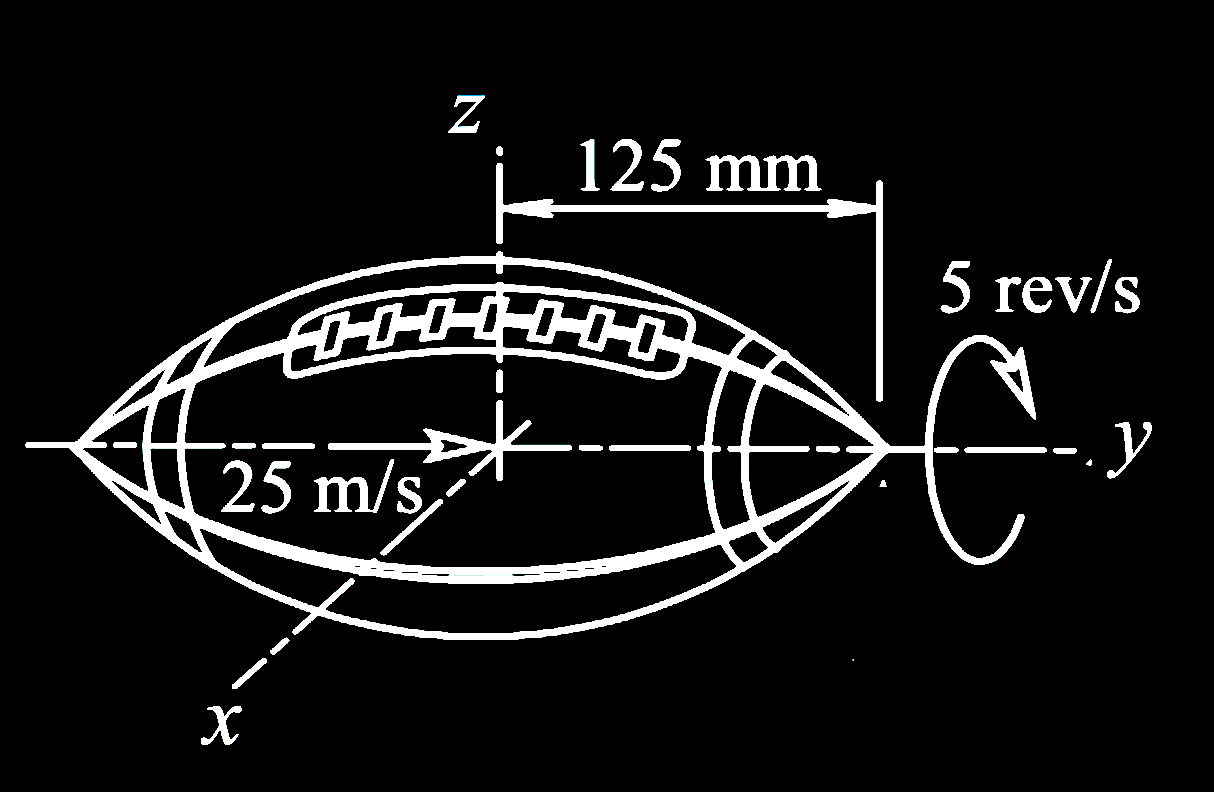
\includegraphics[scale=0.4,frame]{images/problem_1.png}
  %  \caption{Problem 2: 5 rev/s is applied to part (b).}
\end{figure}

\subsubsection*{A football of mass m is flying at a velocity of 25 m/s along the y-axis of the body fixed frame.
The radii of gyration about the axes of the body-fixed frame are 40 mm and 70 mm along the $\bm{x}$-/$\bm{z}$-and the $\bm{y}$-axis, respectively.}

The inertia properties of the football, given the radii of gyration given in the prompt are are:

\begin{equation*}
  \begin{aligned}
    I_b
    &= \left[\begin{array}{ccc}
      m (0.04)^2 & 0 & 0\\
      0 & m (0.07)^2 & 0\\
      0 & 0 & m (0.04)^2
      \end{array}\right]\\
    &= m\left[\begin{array}{ccc} 0.0016 & 0 & 0\\ 0 & 0.0049 & 0\\ 0 & 0 & 0.0016 \end{array}\right]
  \end{aligned}
\end{equation*}

\subsubsection*{(a) Compute the kinetic energy of the ball.
Use the $\bm{ZYZ}$ Euler angles to represent the orientation of the ball.}

The translational kinetic energy is computed as:

$$ T_\text{trans} = \frac{1}{2}m\left( v \cdot v \right) $$

Where $v = [0,25,0]^T$ m/s, the translational kinetic energy is:

$$ T_\text{trans} = 312.5\,m \ \ \left[\text{kg}\left(\frac{\text{m}}{\text{s}}\right)^2\right] =  312.5\,m \ \ \left[\text{J}\right] $$

Using the $ZYZ$ Euler angles to represent the orientation of the ball:


\begin{equation*}
  \begin{aligned}
    R_{ZYZ} &= R_{Z}(\psi) R_{Y}(\theta) R_{Z}(\phi) \\
    &= \left[\begin{array}{ccc} \cos\left(\psi \right) & -\sin\left(\psi \right) & 0\\ \sin\left(\psi \right) & \cos\left(\psi \right) & 0\\ 0 & 0 & 1 \end{array}\right]
    \left[\begin{array}{ccc} \cos\left(\theta \right) & 0 & \sin\left(\theta \right)\\ 0 & 1 & 0\\ -\sin\left(\theta \right) & 0 & \cos\left(\theta \right) \end{array}\right]
    \left[\begin{array}{ccc} \cos\left(\phi \right) & -\sin\left(\phi \right) & 0\\ \sin\left(\phi \right) & \cos\left(\phi \right) & 0\\ 0 & 0 & 1 \end{array}\right]\\
    &= \footnotesize{\left[\begin{array}{ccc}
      \cos \left(\phi \right)\,\cos \left(\psi \right)\,\cos \left(\theta \right)-\sin \left(\phi \right)\,\sin \left(\psi \right) & -\cos \left(\phi \right)\,\sin \left(\psi \right)-\cos \left(\psi \right)\,\cos \left(\theta \right)\,\sin \left(\phi \right) & \cos \left(\psi \right)\,\sin \left(\theta \right)\\
      \cos \left(\psi \right)\,\sin \left(\phi \right)+\cos \left(\phi \right)\,\cos \left(\theta \right)\,\sin \left(\psi \right) & \cos \left(\phi \right)\,\cos \left(\psi \right)-\cos \left(\theta \right)\,\sin \left(\phi \right)\,\sin \left(\psi \right) & \sin \left(\psi \right)\,\sin \left(\theta \right)\\
      -\cos \left(\phi \right)\,\sin \left(\theta \right) & \sin \left(\phi \right)\,\sin \left(\theta \right) & \cos \left(\theta \right)
      \end{array}\right]}
  \end{aligned}
\end{equation*}


Where computing the body angular velocity:

$$ \omega_b = \textbf{vect}\left(  R^T \dot{R} \right) =
\left<\begin{array}{c} \sin\left(\phi \right)\,\dot{\theta} -\cos\left(\phi \right)\,\sin\left(\theta \right)\,\dot{\psi} \\ \cos\left(\phi \right)\,\dot{\theta} +\sin\left(\phi \right)\,\sin\left(\theta \right)\,\dot{\psi} \\ \cos\left(\theta \right)\,\dot{\psi} +\dot{\phi}  \end{array}\right>$$

The rotational kinetic energy is computed as:

\begin{equation*}
  \begin{aligned}
    T_\text{rot} &= \frac{1}{2} \omega_b^T I_b\, \omega_b \\
      &= \frac{m}{20000}\left(16\,\dot{\phi}^2+49\,\,\dot{\psi}^2+16\,\dot{\theta}^2-33\,\,{\cos\left(\phi \right)}^2\,\dot{\psi}^2+33\,\,{\cos\left(\phi \right)}^2\,\dot{\theta}^2-33\,\,{\cos\left(\theta \right)}^2\,\dot{\psi}^2\right. \\
      & \ \ \ \ \ \ \ \ \ \ \ \ \ \ \ \ \ \ \left.+33\,\,{\cos\left(\phi \right)}^2\,{\cos\left(\theta \right)}^2\,\dot{\psi}^2+32\,\cos\left(\theta \right)\,\dot{\psi} \,\dot{\phi} +66\,\,\cos\left(\phi \right)\,\sin\left(\phi \right)\,\sin\left(\theta \right)\,\dot{\theta} \,\dot{\psi}\right)
  \end{aligned}
\end{equation*}

The total kinetic energy is:

\begin{answer}
\begin{equation*}
  \begin{aligned}
    T &= T_\text{trans} + T_\text{rot} \\
      &= 312.5\,m \ +\\
      & \ \ \ \ \  \frac{m}{20000}\left(16\,\dot{\phi}^2+49\,\,\dot{\psi}^2+16\,\dot{\theta}^2-33\,\,{\cos\left(\phi \right)}^2\,\dot{\psi}^2+33\,\,{\cos\left(\phi \right)}^2\,\dot{\theta}^2\right. \\ 
      & \ \ \ \ \ \ \ \ \ \ \ \ \ \ \ \ \ \ -33\,\,{\cos\left(\theta \right)}^2\,\dot{\psi}^2 +33\,\,{\cos\left(\phi \right)}^2\,{\cos\left(\theta \right)}^2\,\dot{\psi}^2+32\,\cos\left(\theta \right)\,\dot{\psi} \,\dot{\phi} \\
      & \ \ \ \ \ \ \ \ \ \ \ \ \ \ \ \ \ \ \left. +66\,\,\cos\left(\phi \right)\,\sin\left(\phi \right)\,\sin\left(\theta \right)\,\dot{\theta} \,\dot{\psi}\right)
  \end{aligned}
\end{equation*}
\end{answer}

\subsubsection*{(b) If the ball is spinning about the y-axis of the body-fixed frame at 5 rev/s,
as shown in the figure,
what is the kinetic energy?}

If the ball is spinning about the y-axis of the body-fixed frame at 5 rev/s,
as shown in the figure, we can state that the body angular velocity is:

$$ \omega_b = \left<\begin{array}{c} 0 \\ 5 \\ 0  \end{array}\right>\ \  \left[\frac{\text{rev}}{\text{s}} \right] =
\left<\begin{array}{c} 0 \\ 10 \pi \\ 0  \end{array}\right>\ \  \left[\frac{\text{rad}}{\text{s}} \right]$$

For this body rate, the rotational kinetic energy is:

\begin{equation*}
  \begin{aligned}
    T_\text{rot} &= \frac{1}{2} \omega_b^T I_b\, \omega_b \\
      &= 0.245\,m\,\pi^2 \ \ \left[\text{kg}\left(\frac{\text{m}}{\text{s}}\right)^2\right]\\
      &= 0.245\,m\,\pi^2 \ \ \left[ J \right]
  \end{aligned}
\end{equation*}

The pairing this with the translational kinetic energy from part (a), the total kinetic energy is:

\begin{answer}
\begin{equation*}
  \begin{aligned}
    T = T_\text{trans} + T_\text{rot} = \left(312.5\,m +  0.245\,m\,\pi^2\right) \ \  \left[ J \right]
  \end{aligned}
\end{equation*}
\end{answer}

The following MATLAB script was used to solve this problem:

% \color{white}
\hspace*{6em}\inputminted[frame=leftline,fontsize=\footnotesize,lastline=48]{matlab}
{./matlab/Problem_2.m}
% \color{black} 

% \begin{equation*}
%   \begin{aligned}
%     V &= F \left[ \int_0^L \left( 1 + \frac{1}{2}(w')^2 - \frac{1}{8}(w')^4 \right) dx - \int_0^L 1\ dx \right] + \int_0^L w\,\mu\,g\, dx\\
%       &= F \left[ \int_0^L \left( \frac{1}{2}(w')^2 - \frac{1}{8}(w')^4 \right) dx \right] + \int_0^L w\,\mu\,g\, dx
%   \end{aligned}
% \end{equation*}

% % \color{white}
% \hspace*{6em}\inputminted[frame=leftline,fontsize=\footnotesize,lastline=51]{matlab}
% {./matlab/Problem_2.m}
% % \color{black} 
 
% % \color{white}
% \hspace*{6em}\inputminted[frame=leftline,fontsize=\footnotesize]{matlab}
% {./matlab/Q6_8.m}
% % \color{black} 

% \begin{figure}[H]
%     \centering
%     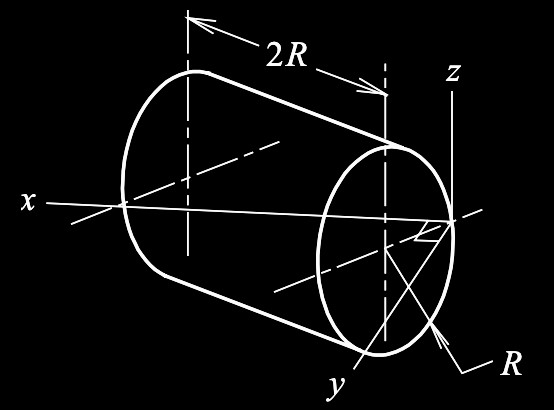
\includegraphics[scale=0.7,frame]{images/Q5_13.png}
% \end{figure}




\end{document}

